\renewcommand{\figurename}{Supplementary Figure}
\setcounter{figure}{0}

\begin{figure}[ht]
  \centering
  % \fbox{\rule[-.5cm]{0cm}{4cm} \rule[-.5cm]{4cm}{0cm}}
  {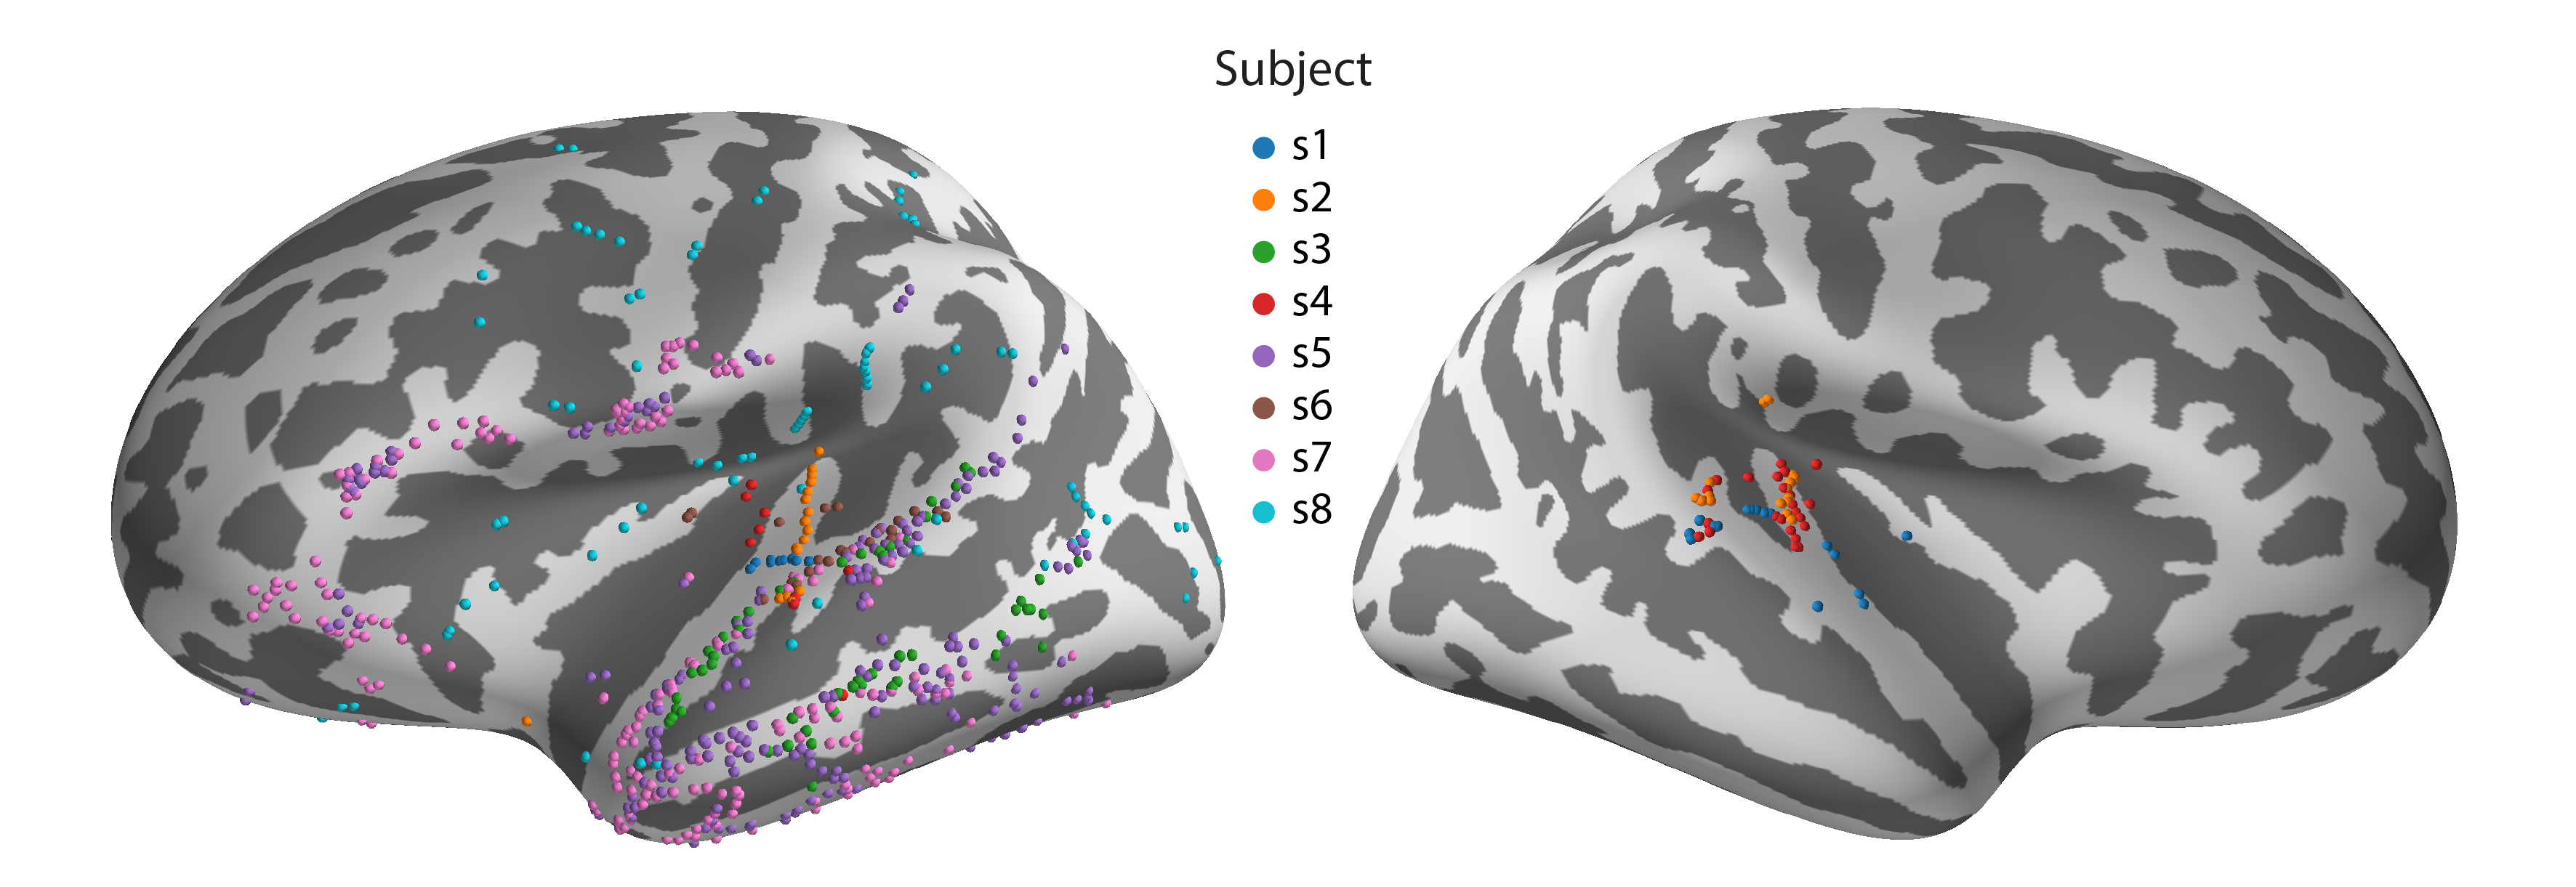
\includegraphics[width=0.95\linewidth]{supplementary_figures/Figure_supplemental_subject_ID_727-01.png}}
  \caption{Subject-wise electrode localization. Electrodes are plotted on the inflated Freesurfer average brain and are colored by their corresponding subject identity.}
  \label{fig:s1}
\end{figure}


\begin{figure}[ht]
  % \centering
  % \fbox{\rule[-.5cm]{0cm}{4cm} \rule[-.5cm]{4cm}{0cm}}
  {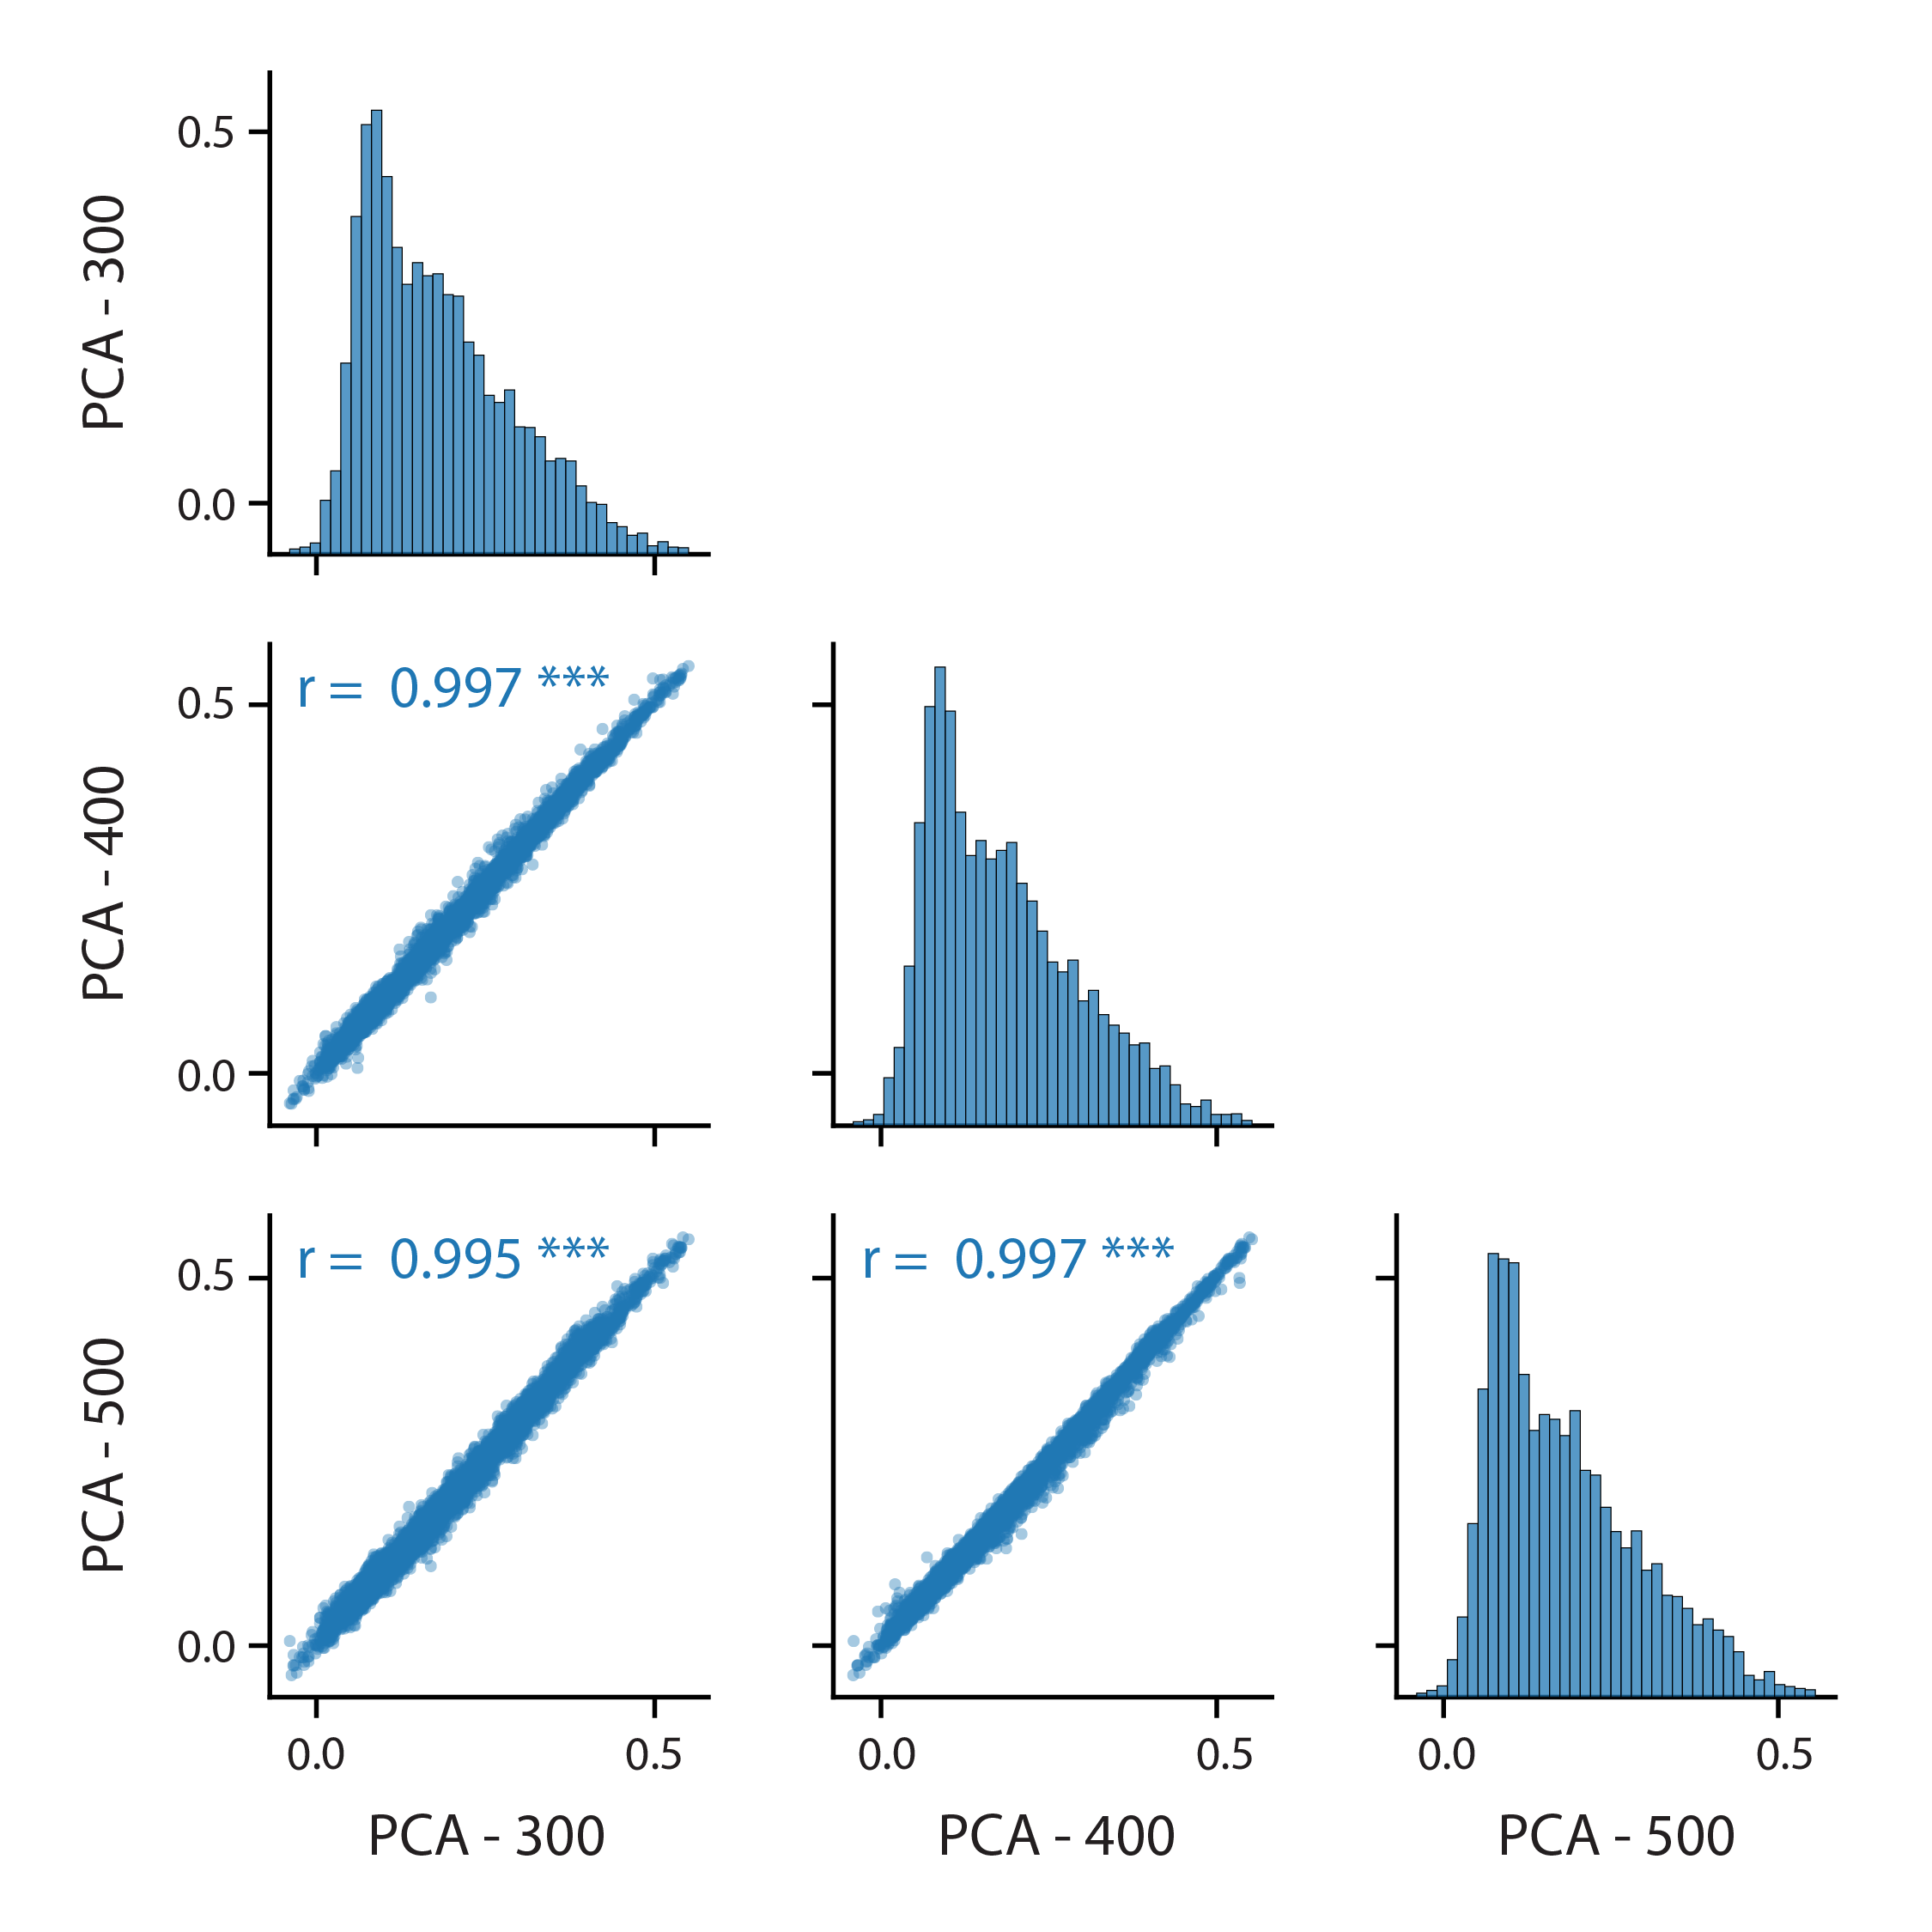
\includegraphics[width=0.47\linewidth]{supplementary_figures/Figure_supplemental_change_PCA-01.png}}
  {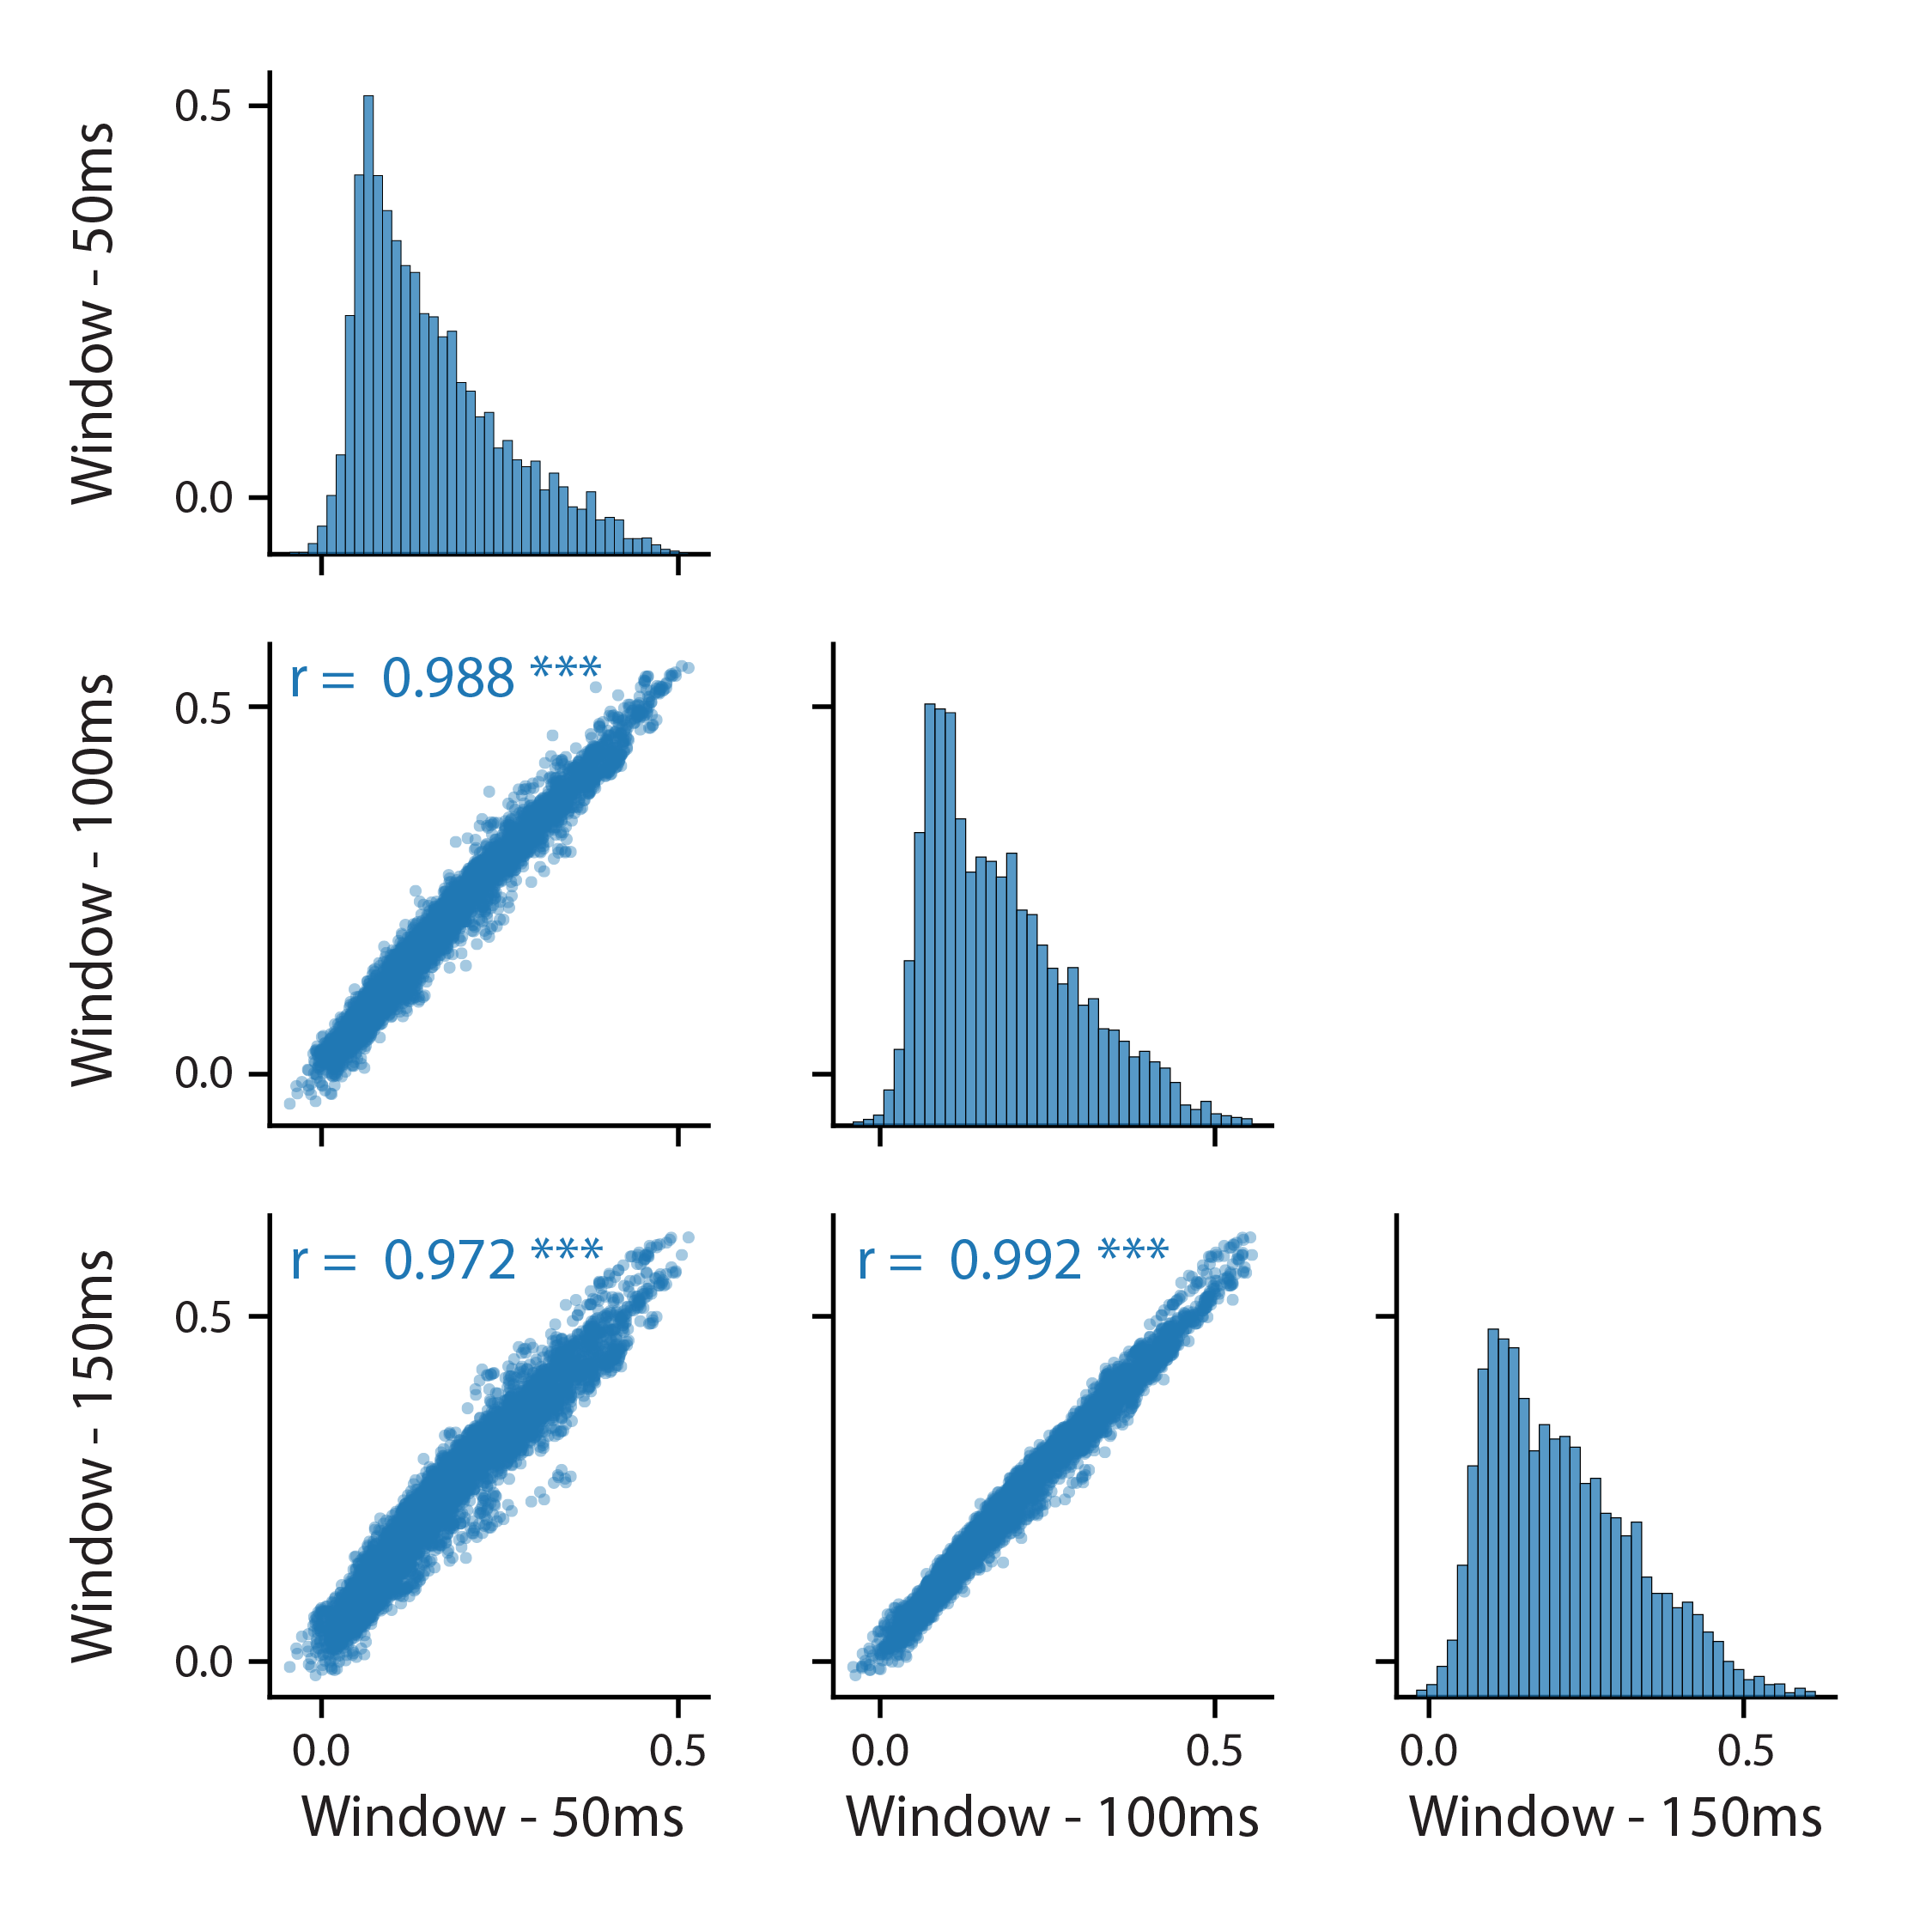
\includegraphics[width=0.47\linewidth]{supplementary_figures/Figure_supplemental_change_Window-01.png}}
  % {\includegraphics[width=0.95\linewidth]{supplementary_figures/Figure_supplemental_change_PCAplusWindow.pdf}}
  \caption{Effect of regression hyperparameters on scores. The left plot shows the pairwise effects on the peak brain similarity scores when altering the number of principal components of the LLM embeddings used for computing scores with ridge regression, keeping a $100$ms window size constant. The right plot shows the pairwise effects of altering the width of the averaging window around word centers for estimating neural responses to words, keeping the PCA dimensionality of $500$ constant. Along each plot’s diagonal is the marginal distribution for that hyperparameter setting. The off-diagonal plots display scatter plots of all the peak-scores for all models together for one hyperparameter setting against another. Each dot represents the peak brain correlation score for one model-electrode pair. All pairs of settings produce scores which are highly correlated, as written in each subplot (Pearson correlation, *** indicates $p<0.001$).}
  \label{fig:s2}
\end{figure}

\begin{figure}[ht]
  \centering
  % \fbox{\rule[-.5cm]{0cm}{4cm} \rule[-.5cm]{4cm}{0cm}}
  {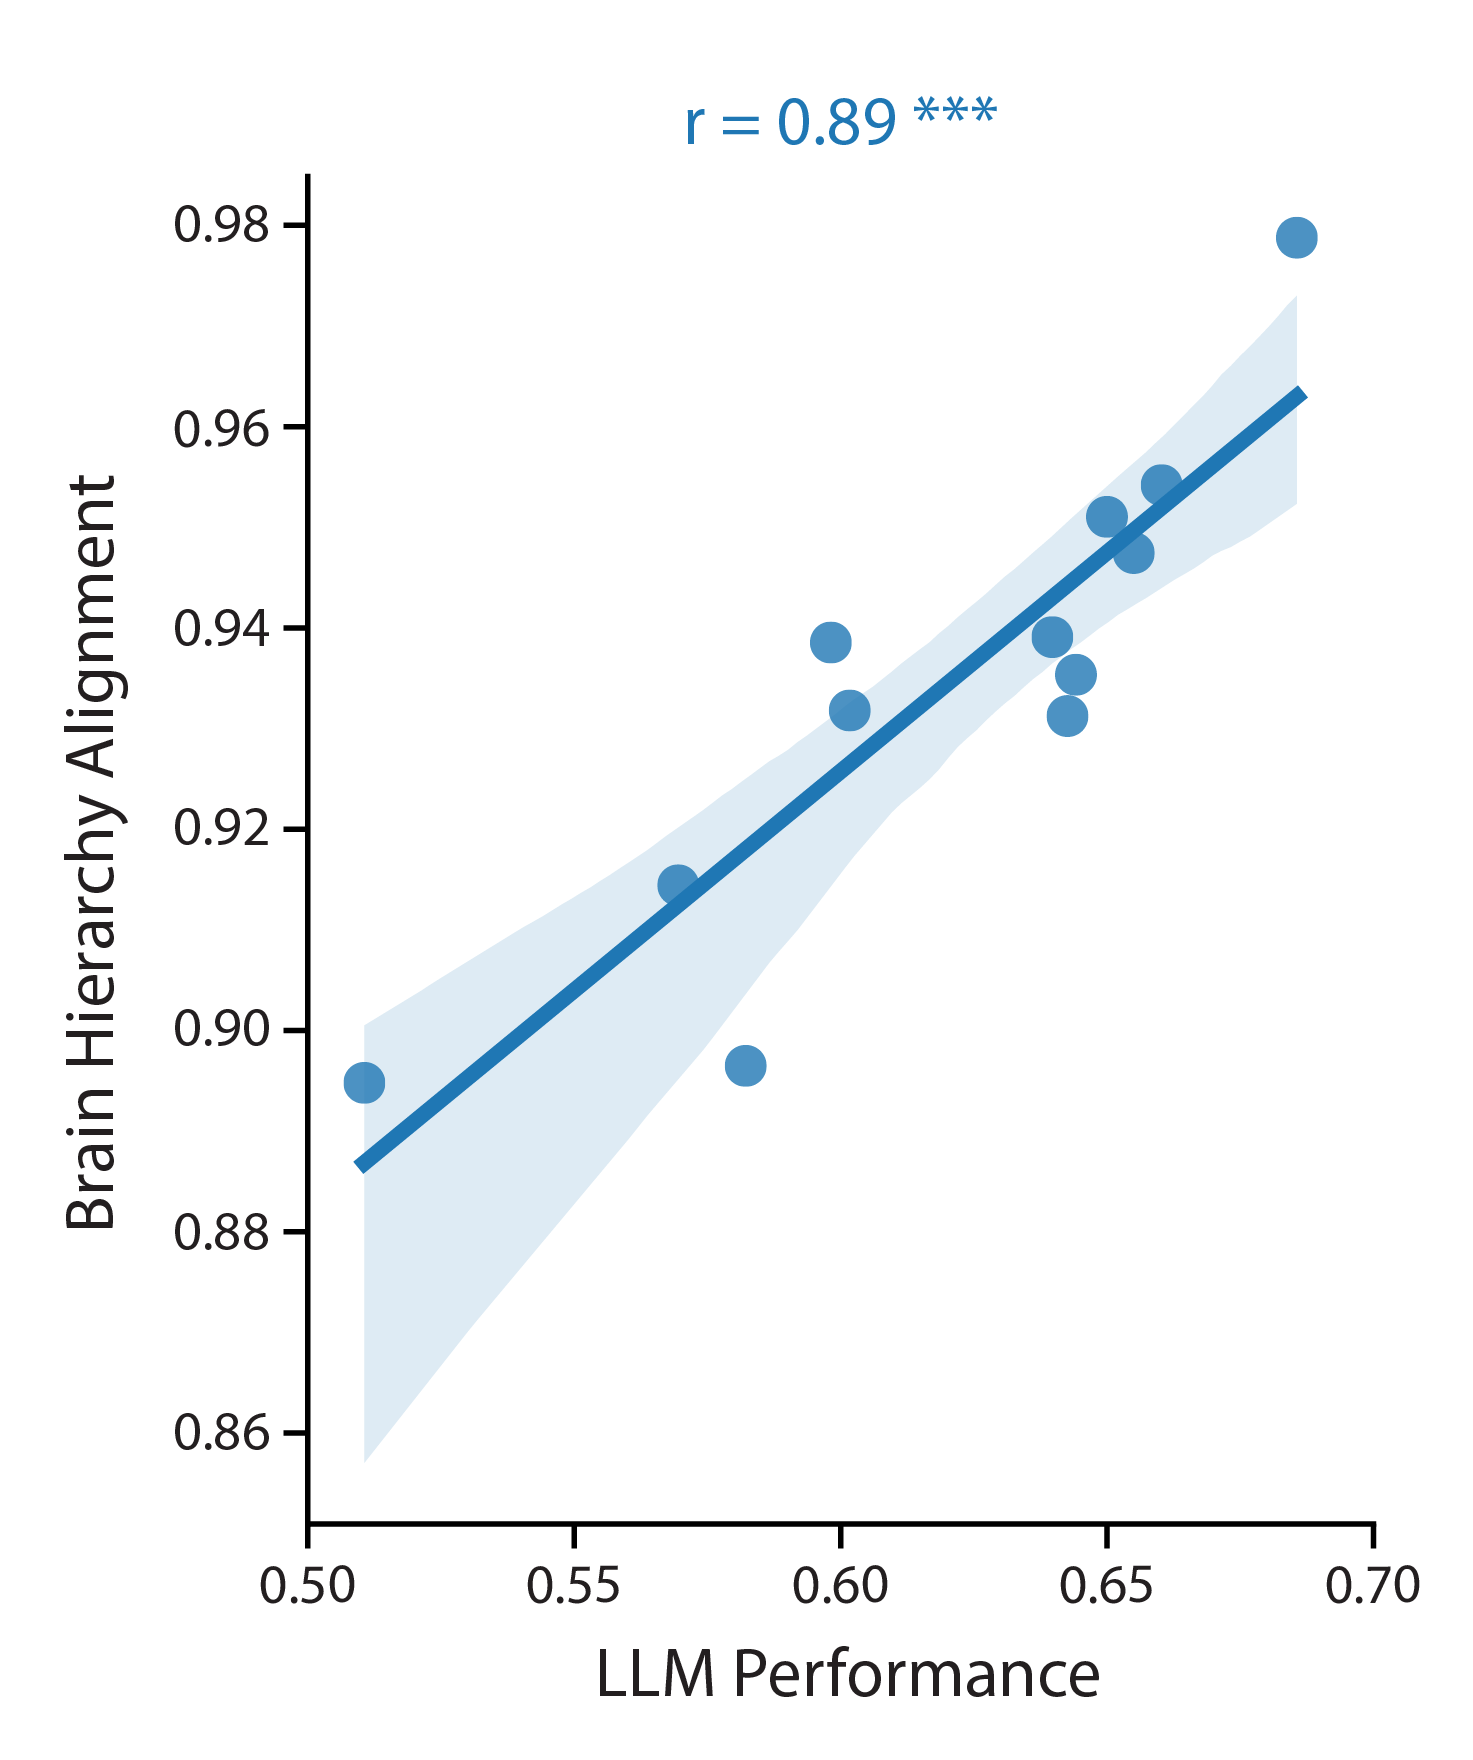
\includegraphics[width=0.45\linewidth]{supplementary_figures/Figure_supplemental_hierarchy_vs_performance_LAGTRF1D-01.png}}
  \caption{Hierarchy alignment by model when using electrode lag instead of distance to estimate neural hierarchy. We used the electrode lag, instead of distance from primary auditory cortex, to bin electrodes into a hierarchy with a bin-width of 40ms. We estimated electrode lag using the peak of a 1D temporal receptive field fitted for each electrode to predict its response from the acoustic envelope of the stimulus sound. We then performed the same analysis as shown in Fig. \protect\ref{fig:3}, reproducing Fig. \protect\ref{fig:3}B with new brain hierarchy alignment for each model. These alignment values are similarly significantly correlated with LLM performance (Pearson $r=0.89, p=0.0001$).}
  \label{fig:s3}
\end{figure}

\begin{figure}[ht]
  \centering
  % \fbox{\rule[-.5cm]{0cm}{4cm} \rule[-.5cm]{4cm}{0cm}}
  {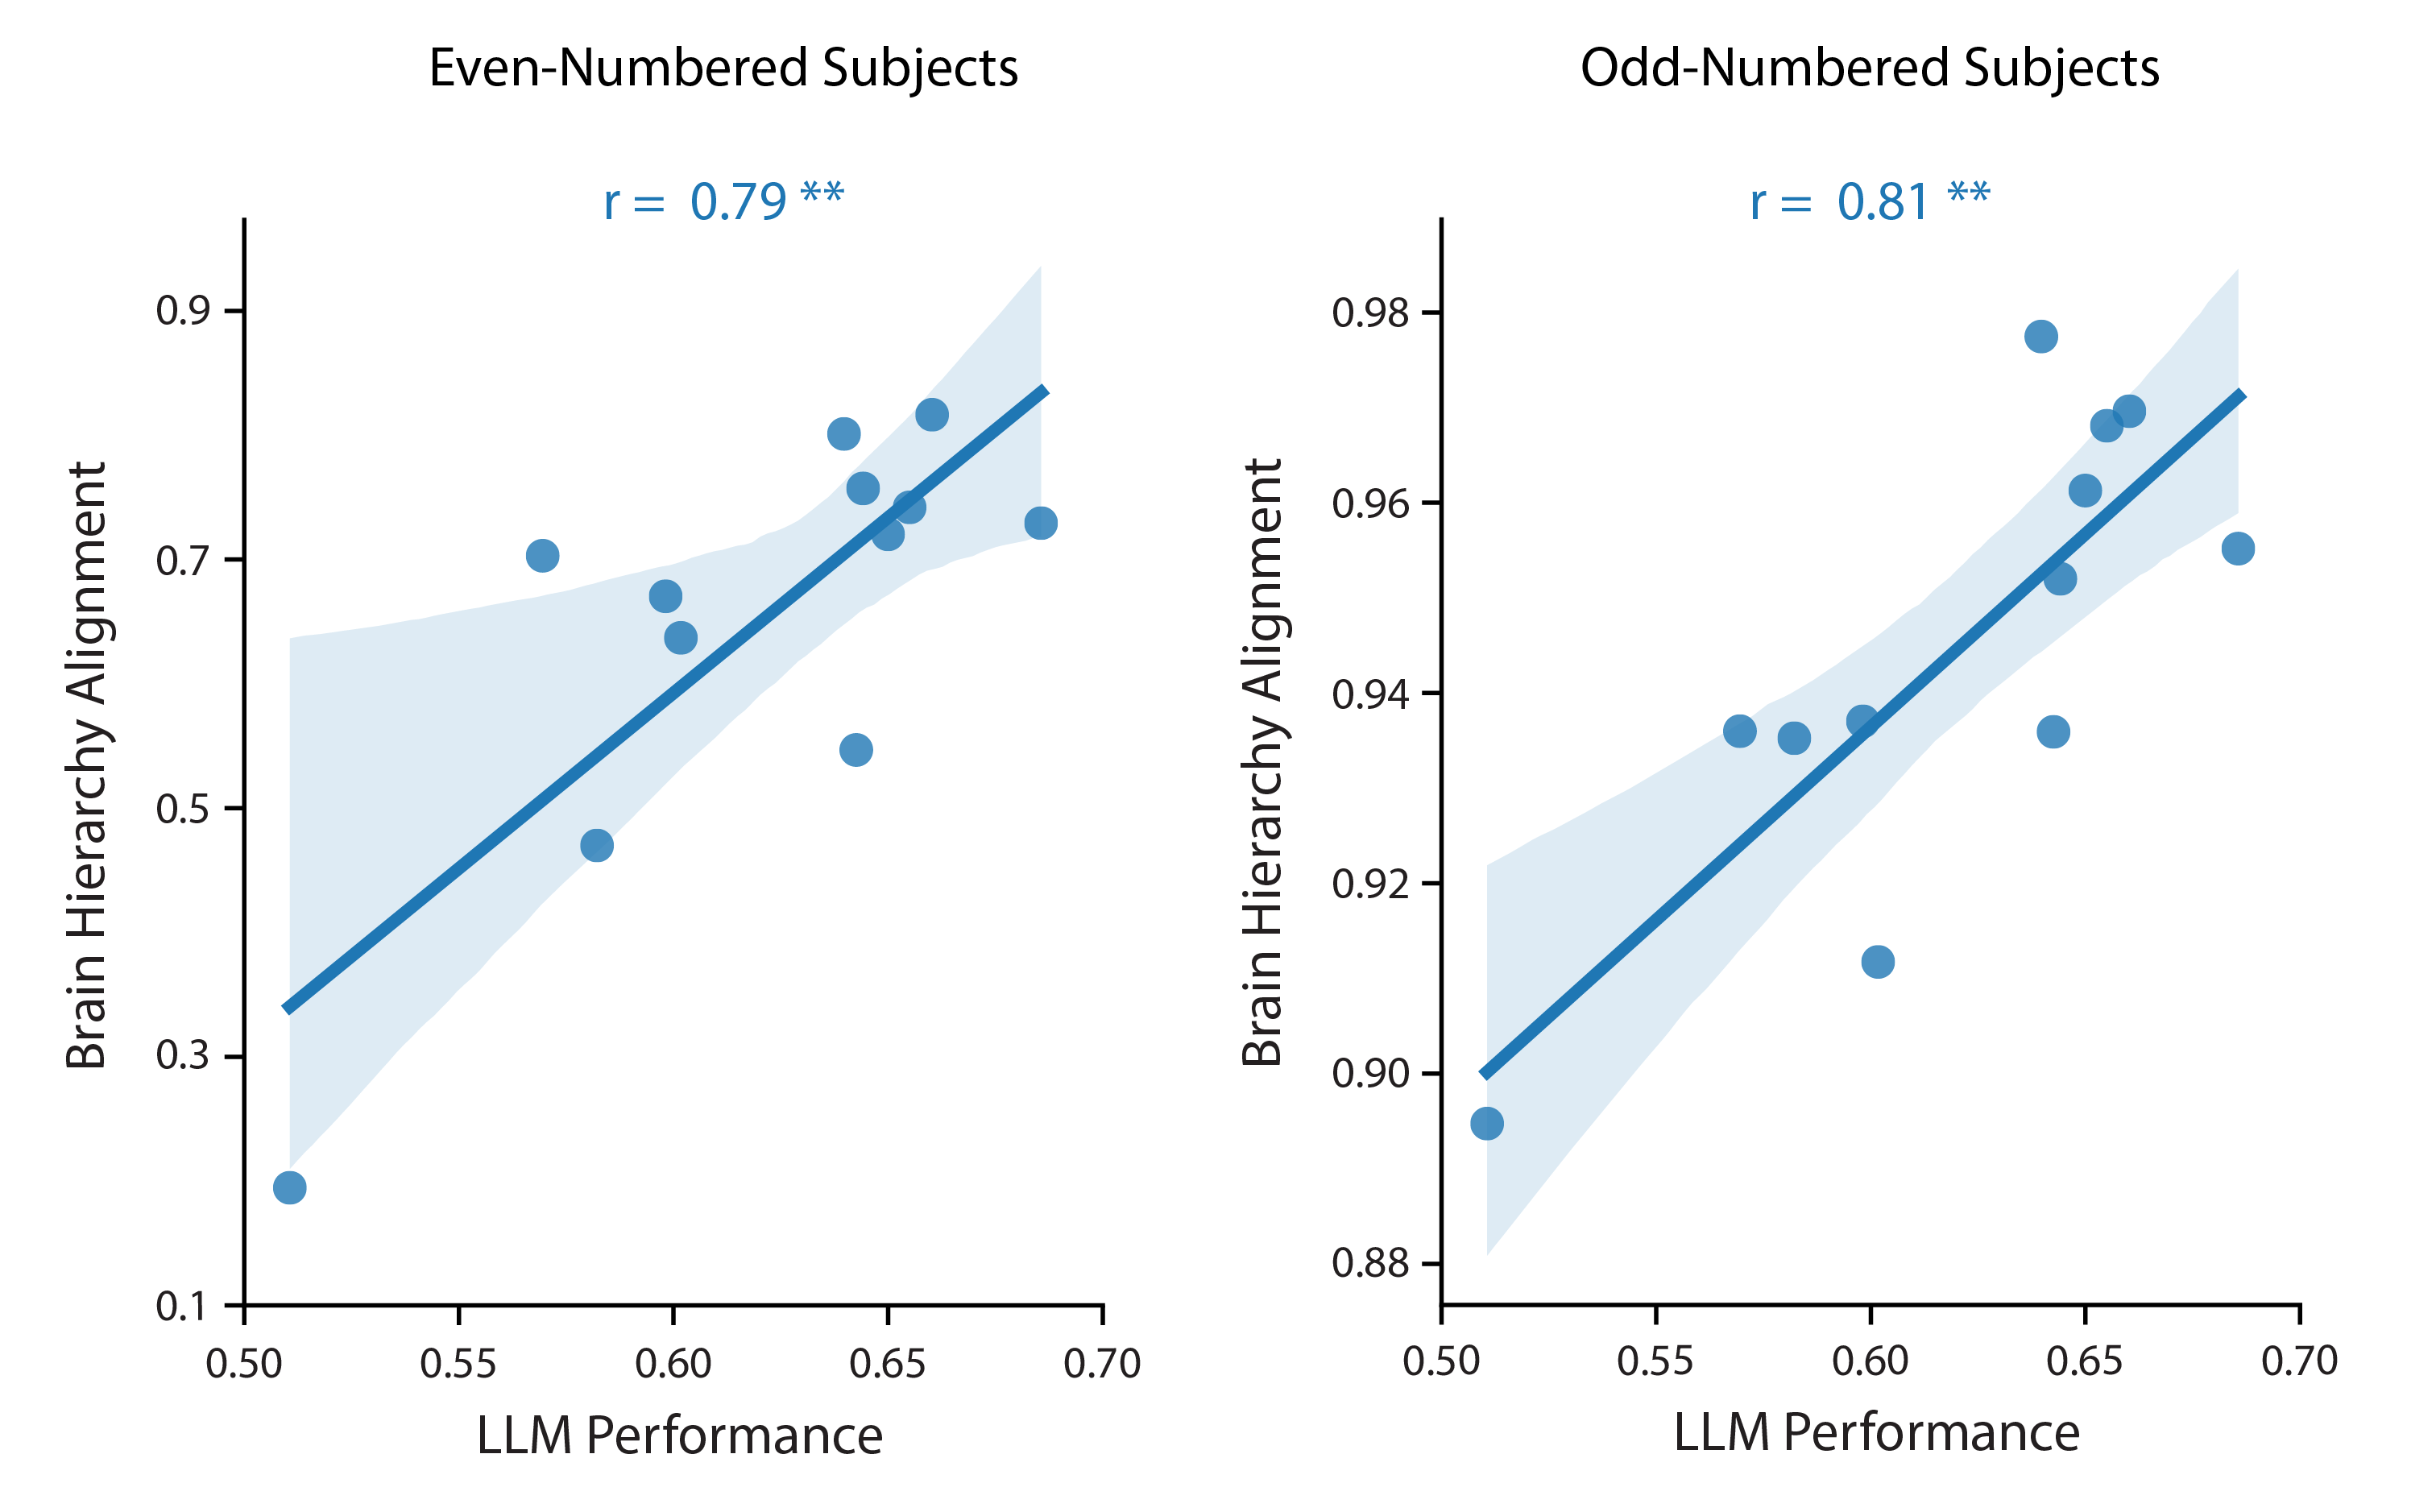
\includegraphics[width=0.95\linewidth]{supplementary_figures/Figure_supplemental_hierarchy_vs_performance_DISTANCE_Even-and-Odd-01.png}}
  \caption{Hierarchy alignment patterns hold for partial subject groupings. Splitting the electrodes based on whether they came from even- or odd-numbered subjects, we performed the same analyses as in Fig. \protect\ref{fig:3}B. Both subject groups show that brain hierarchy alignment is significantly correlated with LLM performance (Pearson correlations in figure, even $p=0.0022$, odd $p=0.0013$) demonstrating that this effect is not the result of a single outlier subject.}
  \label{fig:s4}
\end{figure}